\section{The DOM: The Basic Unit of IceCube}

\label{subsec:pmt}
\subsection{The Photomultiplier Tube}
The basic unit of the IceCube detector is the \emph{digital optical module}, often referred to simply as the \emph{DOM} \cite{Description-IceCube}.
The DOM is designed around a downward-facing 10 inch R7081-02 photomultiplier tube (\emph{PMT}) from Hammamatsu Photonics \cite{IceCube-PMT,IceCube-PMT-Hammamatsu} and includes onboard electronics for standard operation as shown in Figure~\ref{fig:icecube_dom}. 
Circuit boards are included for data acquisition, control, calibration, comminuications and power conversion as well as for high voltage input from the surface.
The electronics of the DOM are encased in a spherical glass housing designed to withstand the high pressures associated with operation in the glacier of Antarctica.
The PMT is optically coupled to the glass housing in order to minimize distortion of incoming light. 

\begin{figure}
\centering
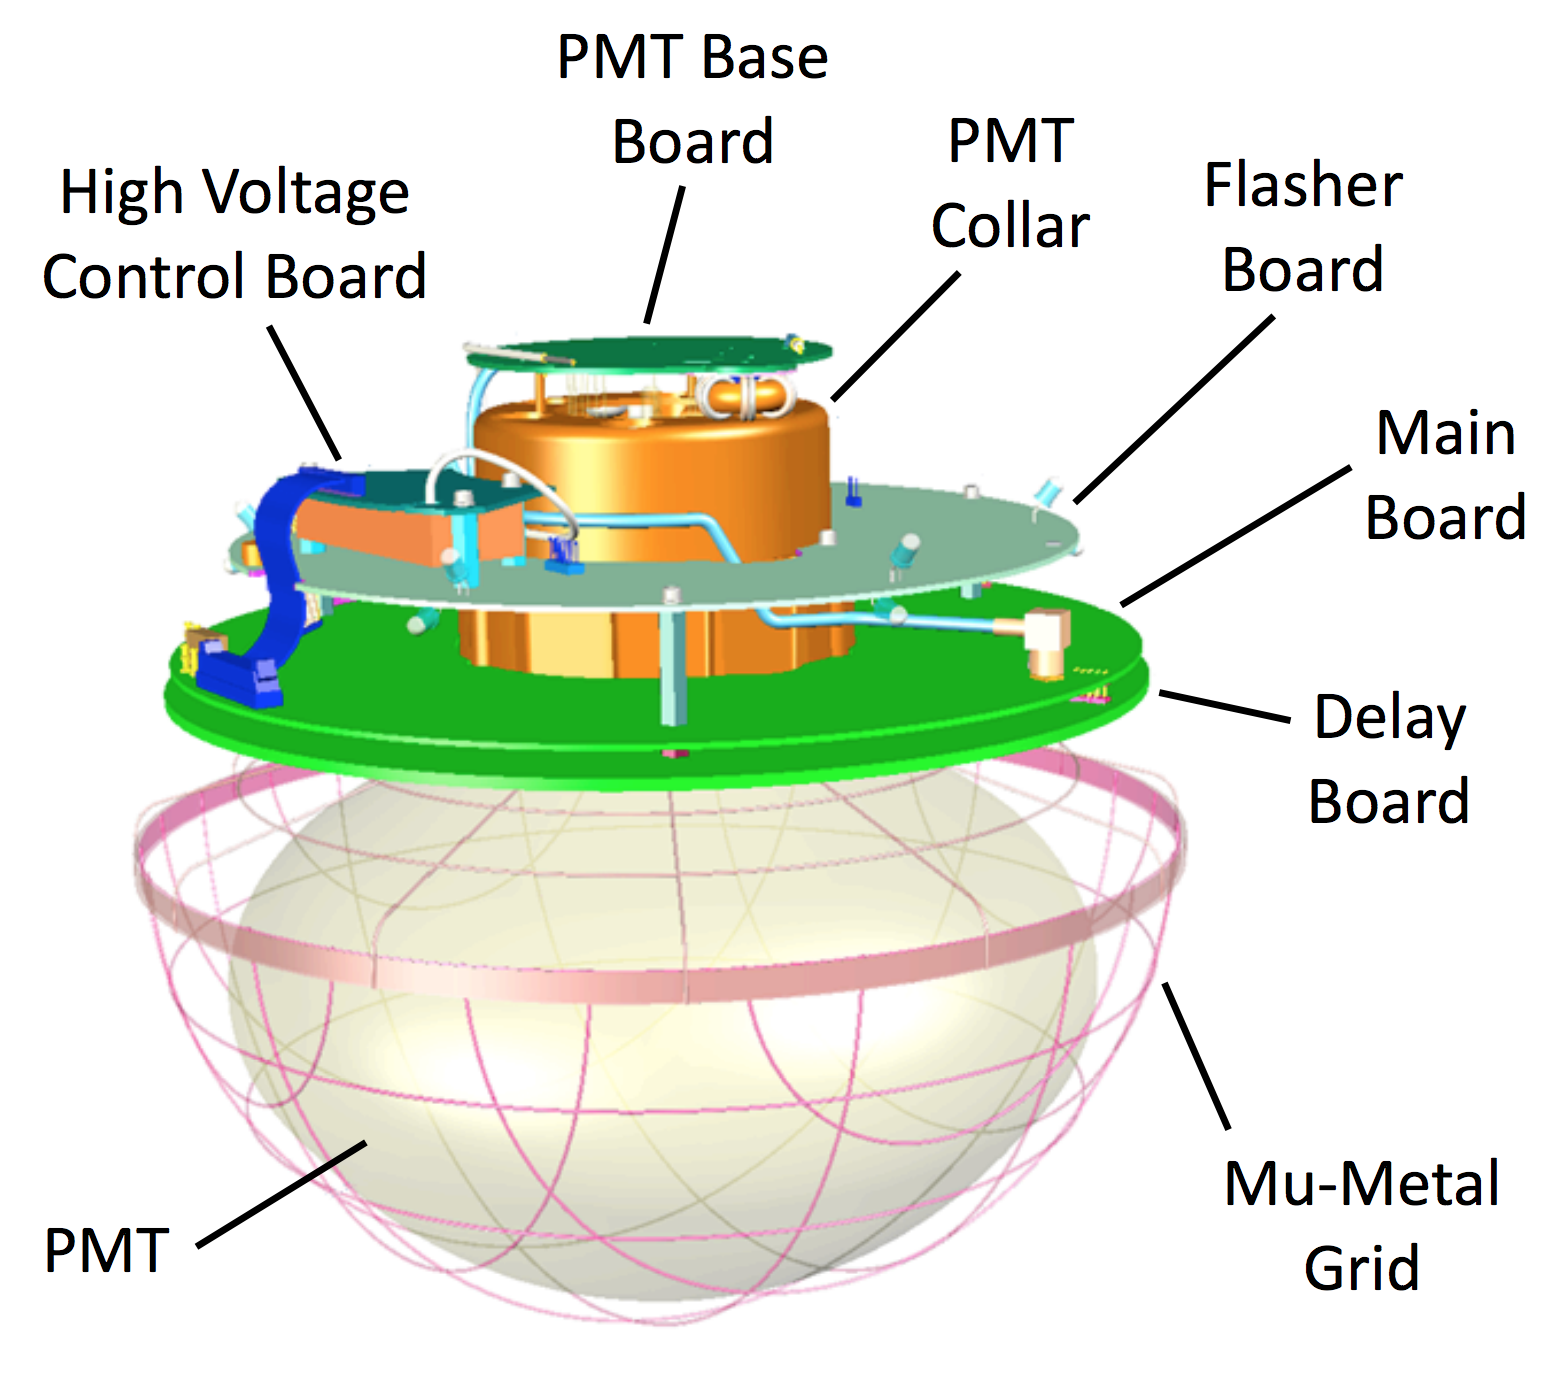
\includegraphics[width=0.4\textwidth]{icecube_dom.png}
\caption{The IceCube DOM contains multiple components, including the PMT itself as well as various electronics necessary for semi-autonomous operation.}
\label{fig:icecube_dom}
\end{figure}

\label{subsubsec:pulsing}
\subsubsection{Pre-, Late-, and Afterpulsing}
Measurement with the IceCube photomultiplier tubes introduces known effects in the recorded charge.
These effects are divided into \emph{pre-pulses}, \emph{late-pulses}, and \emph{afterpulses}.

\begin{figure}
\centering
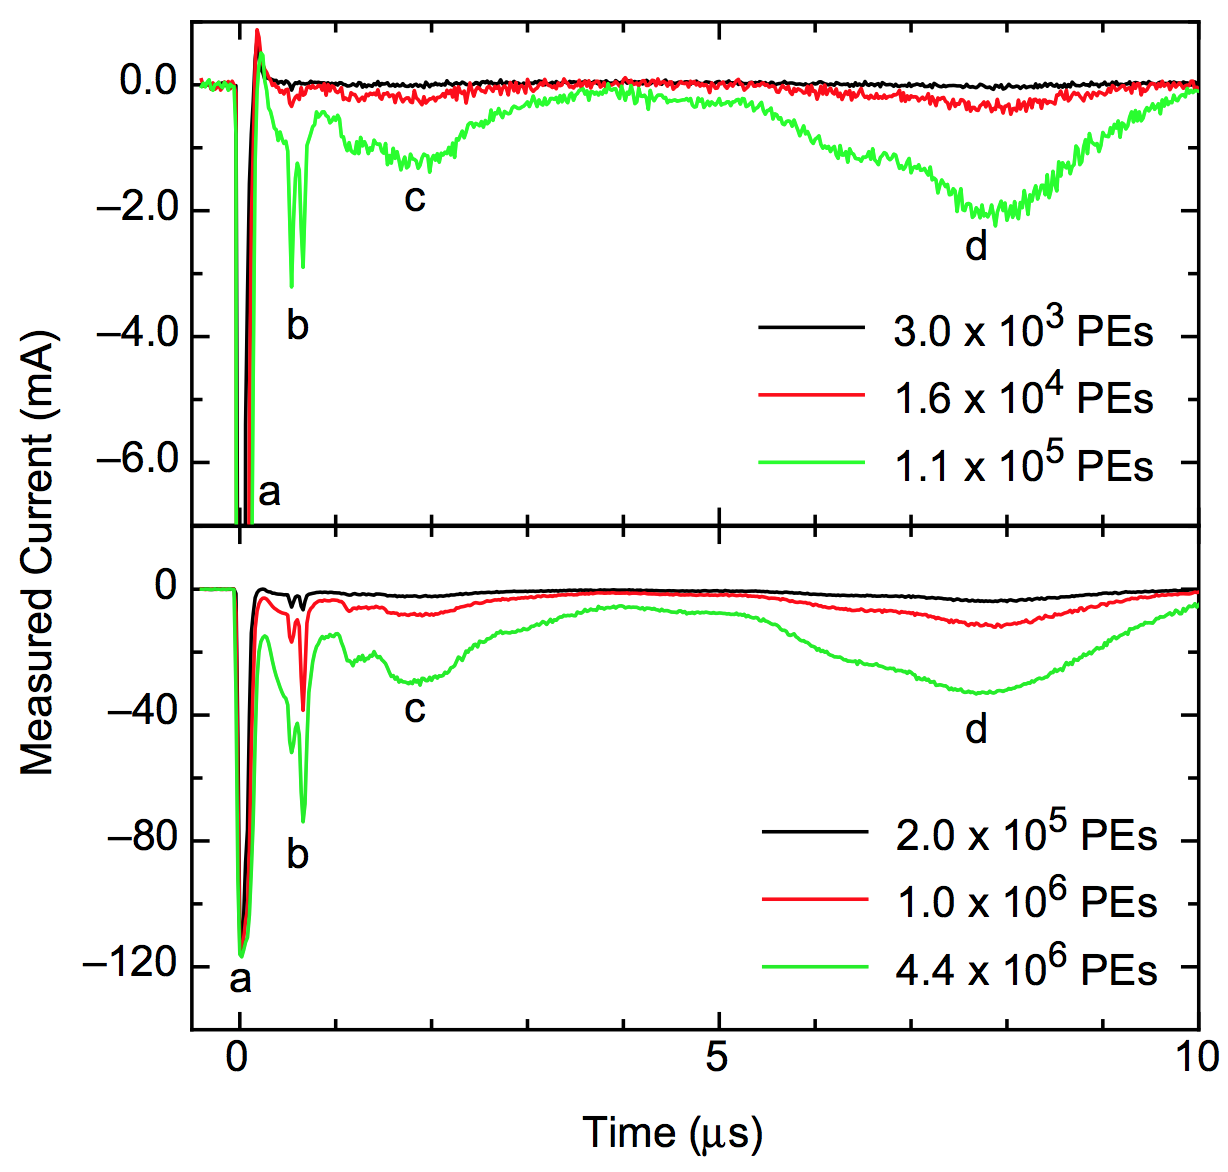
\includegraphics[width=0.4\textwidth]{afterpulsing.png} 
\caption{Afterpulsing calibration measurements performed in the lab. LEDs with known brightness were flashed to test for off–time response of the IceCube PMT. Clear dips, corresponding to detected charge, are visible. Drop (a) corresponds to the initial LED flash while (b), (c), and (d) show prominant afterpulsing peaks. Image taken from \cite{IceCube-PMT}.}
\end{figure}
The pre-pulses, arriving within a few dozens of nanoseconds prior to the main signal, are thought to arise from the small probability of an electron bypassing one of the dynodes. 
Late-pulses are likewise thought to be produced by electrons which return to a previous dynode, inducing a signal a few dozens of nanoseconds immediately following the main signal.
These signals tend to be small and inconsequential for physics measurements.

After-pulses, which arise from ionization of residual gases in the PMT, are a more significant concern for calibration work as addressed in Section~\ref{sec:vuvuzela_limitations}.
The ionized atoms tend to travel significantly more slowly than electrons, resulting in a  delay between the main signal and the subsequent afterpulses that may be as large as 10 microseconds.

\label{ubsec:discriminator}
\subsection{The Discriminator Used for DOM Triggering}
A discriminator onboard the DOM is used to identify signals from the PMT with a voltage threshold corresponding to 0.25 photoelectrons (\emph{PE}).
Each discriminator crossing begins a \emph{DOM launch}, the lowest level signal available in the IceCube detector containing a representation of the raw PMT output in the form of a \emph{waveform}.
Launches are stored in DOM memory while awaiting a decision from the triggering system.

\label{subsec:LC}
\subsection{Local Coincidence}
If any of the notified DOMs also record a launch within a configurable 1 microsecond window, both launches are said to form a \emph{hard local coincidence} (\emph{HLC}) pair.
Nearby DOMs, here defined to be either of the two DOMs above or below the current DOM, are notified of the launch via a signal sent using the \emph{local coincidence} wiring.
Launches which fail to satisfy the local coincidence conditions are referred to as \emph{soft local coincidence} (\emph{SLC}) hits.
Launches recorded as part of an HLC pair receive a flag. 
This flag may be used to later identify only those launches which satisfy the local coincident conditions, providing a simple, default method of identifying hits likely to be caused by particle interactions in the detector.

\label{subsec:digitization}
\subsection{Digitization}
While awaiting a local coincidence decision, the waveform of a launching DOM is passed to the two onboard digitizers.
Information from the PMT is digitized using the fast analog-to-digital converter (\emph{fADC}), which provides binned information at 40$\times 10^6$ samples/second for for the 6.4 microseconds following the initial DOM launch \cite{Description-IceCube}.
Simultaneously, the \emph{Analog to Digital Waveform Digitizer}, or \emph{ATWD}, will digitize the waveform using 322 bins with 3.3 nanoseconds per bin. 

If a launch satisfies the HLC conditions, the DOM will request the full digitization of the waveforms from both the ATWD and FADC, providing a complete record of the launch.
Examples of digitized waveforms from the ATWD and fADC are shown in Figure~\ref{fig:waveforms}.

When digitizing a signal, the ATWD experiences up to 29 microseconds of deadtime \cite{Description-IceCube}. 
During this time, the secondary ATWD is available to record further pulses, resulting in a total average fractional deadtime per DOM of $\mathtt{2.2 \times 10^{-5}}$ seconds/second.
In addition, each of the two ATWDs possesses three channels with separate gains.
This provides the ability to accurately measure the waveform, even in cases of saturation.
The unsaturated ATWD with the highest gain provides a record for the launch.

If the launch is instead given the SLC label, the information in the ATWD is lost and the FADC instead digitizes only the three bins associated with the largest peak of the waveform.
While this limits the information available for these launches, the lack of associated nearby launching DOMs provides strong evidence that the launch is due to random detector noise.

\begin{figure}
\centering
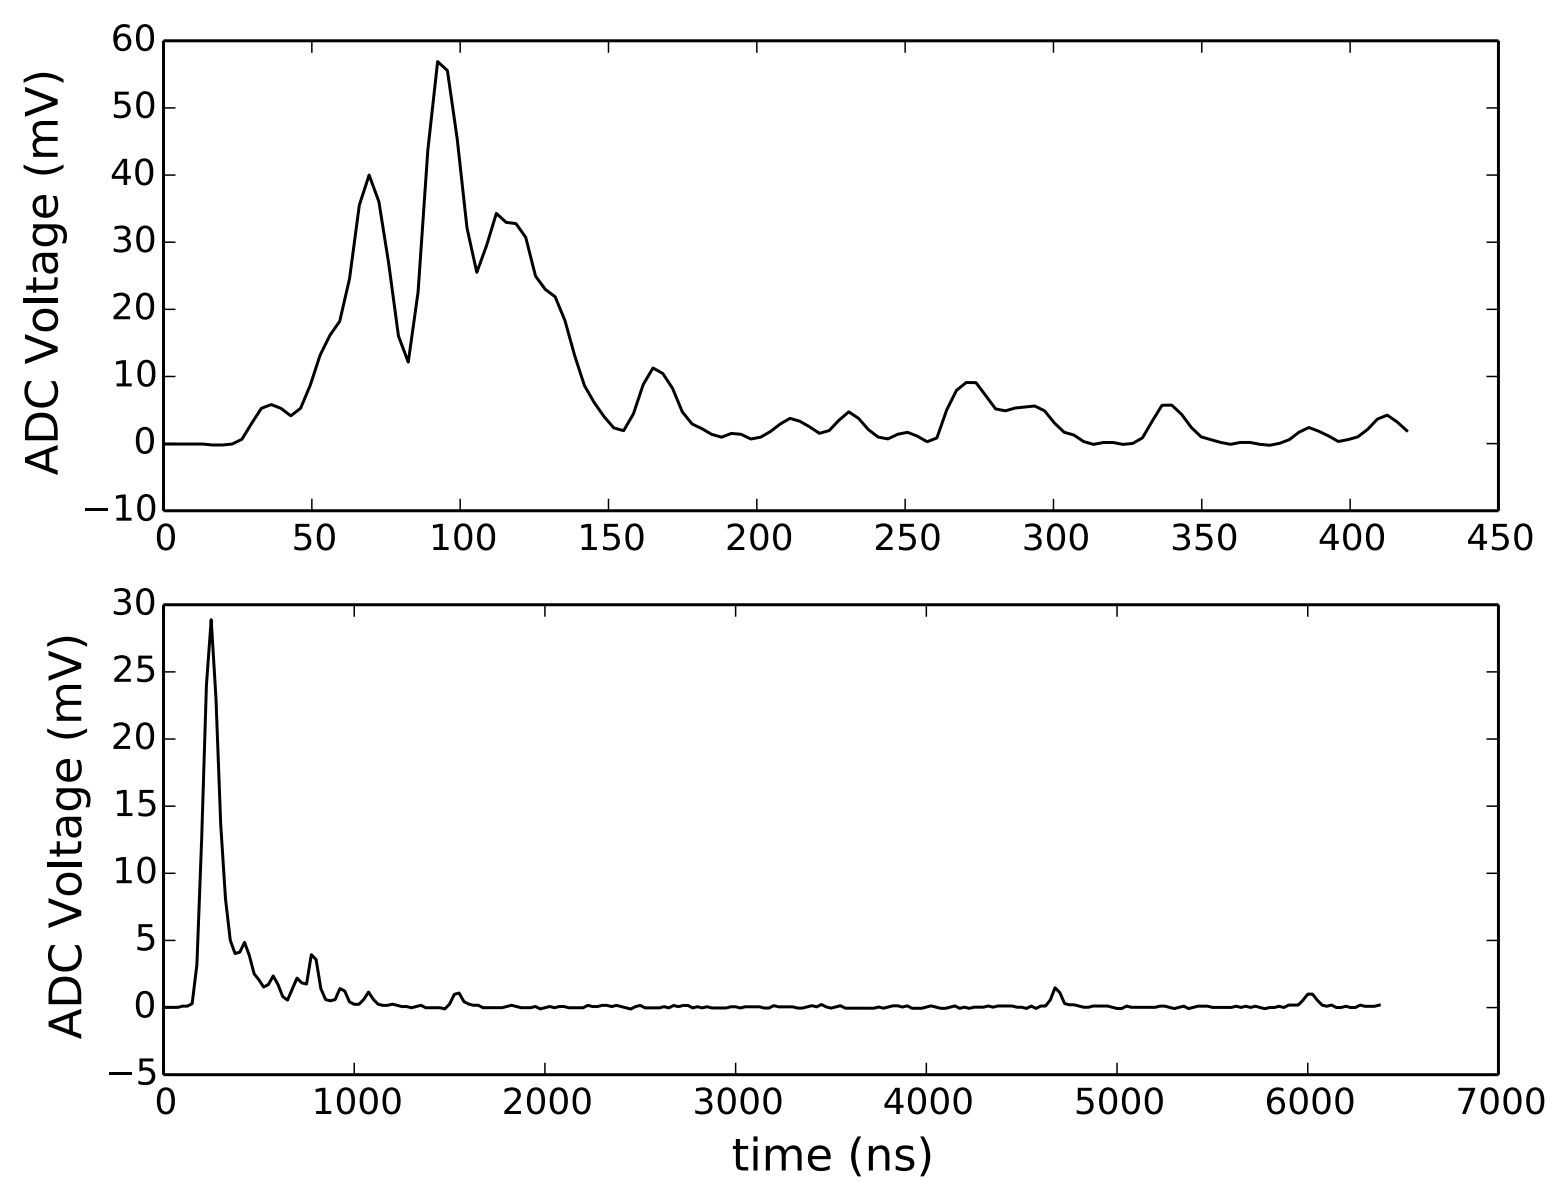
\includegraphics[width=0.6\textwidth]{icecube_waveforms.png}
\caption{Examples of the ATWD (top) and FADC (bottom) waveforms output from an IceCube PMT. Taken from \cite{Description-IceCube}}
\label{fig:waveforms}
\end{figure}

\label{subsec:noise}
\subsection{Noise in IceCube DOMS}
Dedicated measurements using IceCube DOMs have shown multiple components to the detector noise\cite{Thesis-Vuvuzela}. 
A large fraction of the detector noise displays non-Poissonian behavior in time \cite{Description-IceCube}.
The model used in IceCube, shown in Figure~\ref{fig:noise_model}, splits the detector noise into \emph{Poissonian} and \emph{non-Poissonian}(\emph{time-correlated}) noise.

\begin{figure}
\centering
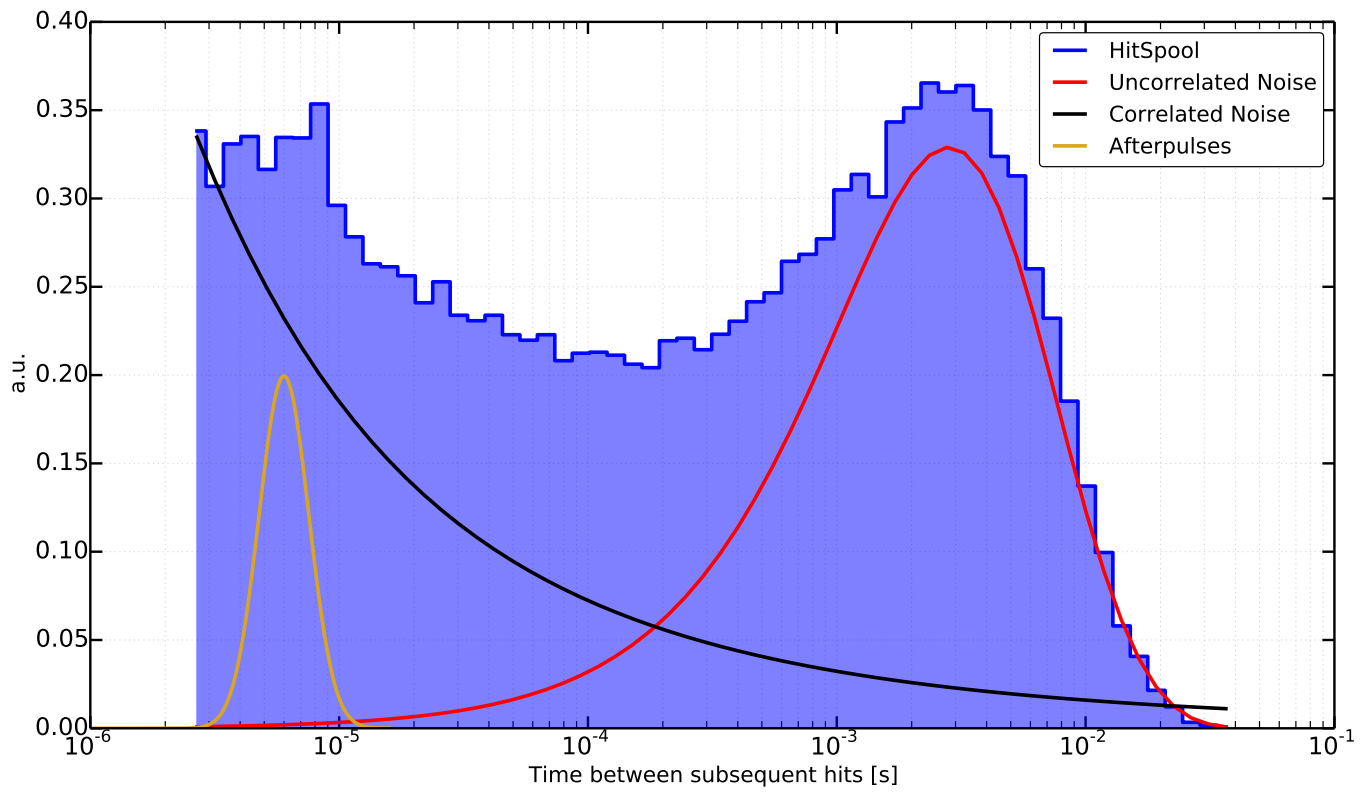
\includegraphics[width=0.6\textwidth]{vuvuzela.png} 
\caption{A histogram of the time between subsequent hits on DOM 15 of string 27. Hitspool data, specialized data collected with no trigger applied, is shown in blue. The "correlated" (non-Poissonian) and "uncorrelated" (Poissonian) features are shown in red and black respectively. The location of a large afterpulsing peak is shown in yellow. Note that the features included are not to scale. Image taken from \cite{Description-IceCube}.}
\label{fig:noise_model}.
\end{figure}

The Poissonian noise consists of thermal noise and radiactive decays in the glass of the PMT and DOM.
Studies of these radioactive components are ongoing, with some evidence that Potassium-40 and Uranium-238 may be responsible for at least some of the observed decays.
Once a decay occurs, a rapid series of pulses occurs in the PMT, leading to a "burst" of noise that continues for up to a few milliseconds \cite{Thesis-Vuvuzela}. 
These hits are believed to be due to a scintillation or luminescence process.

The typical averaged noise rate is 560 Hz for standard IceCube DOMs and 780 Hz for high quantum efficiency DOMs.
Poissonian noise makes up approximately 250 Hz of this rate with the remainder due to non-Poissonian processes.

\label{subsec:triggers}
\subsection{Triggering in IceCube}
Digitized versions of the waveforms are transmitted from the DOM to the IceCube physics data acquisition system (\emph{pDAQ}) for use in trigger and event building.
The most common type of trigger used in IceCube analyses is the \emph{Simple Majority Trigger} or \emph{SMT}. 
This trigger is designed to look for coincidences between DOMs using HLC launches.
Each of the SMTs is defined by three fundamental configurations: a DOMSet, which lists the DOMs available for use in the trigger conditions; a threshold number of HLC launches before the trigger fires; and a time window length in which the HLC are required to coexist.

Once all triggers are identified, a \emph{global trigger} is defined. 
This consists of the superset of all triggers occurring within 10 microseconds of one another.
All detector readout enclosed within the global trigger as well as additional information within an additional 10 microseconds both before and after the trigger is combined into a single \emph{event}.

